\section{Approach: Specification and Design}

The design combines linked borough views, explicit response-time denominators, and a separate station-context analysis.

\subsection{Design Goals and Scope}

The design pursues three primary goals:

\begin{enumerate}
    \item \textbf{Show borough-level response-time disparity with its denominator and spread}, so that a planner can compare the median, p95, incident mix, recorded count, and missing response times (after \cite{hullman2015hops, maceachren2012, padilla2018}).
    \item \textbf{Provide station-related context} from assignment footprints and historical public addresses, with straight-line proximity labelled separately from travel-time coverage.
    \item \textbf{Add mobilisation and historical context} so that incident summaries can be compared with appliance-level records and the 2014 closure cohort identified by \cite{spatial2015}.
\end{enumerate}

Figure~\ref{fig:project-evidence-map} shows how the data sources, processing rules, dashboard, and headline results fit together.

\begin{figure}[H]
\centering
\resizebox{\textwidth}{!}{%
\begin{tikzpicture}[
    stage/.style={draw, rounded corners=1.5pt, align=center, text width=3.3cm, minimum height=2.9cm, font=\scriptsize, inner sep=4pt},
    stat/.style={align=center, text width=3.3cm, font=\scriptsize, inner sep=2pt},
    arr/.style={-{Stealth[length=2.0mm]}, line width=0.45pt},
    node distance=5mm and 5mm
]
\node[stage, fill=blue!8, draw=blue!55!black] (p) {\textbf{Open-data inputs}\\[2pt] incident, mobilisation, borough-boundary, and historical station-address records};
\node[stage, fill=green!8, draw=green!50!black, right=of p] (d) {\textbf{Data treatment}\\[2pt] canonical fields, recorded denominators, matched mobilisations, and spatial checks};
\node[stage, fill=orange!9, draw=orange!65!black, right=of d] (i) {\textbf{Dashboard build}\\[2pt] Python pipeline with provenance sidecars, Flask API, and D3 linked views};
\node[stage, fill=violet!8, draw=violet!60!black, right=of i] (q) {\textbf{Supported use}\\[2pt] borough comparison with denominators and data limitations visible};
\draw[arr] (p) -- (d);
\draw[arr] (d) -- (i);
\draw[arr] (i) -- (q);
\node[stat, below=5mm of p] (s1) {{\large\bfseries 293{,}646}\\ incidents,\\ 2024-01 to 2026-02};
\node[stat, below=5mm of d] (s2) {{\large\bfseries 37.9\,\%}\\ records with\\ precise coordinates};
\node[stat, below=5mm of i] (s3) {{\large\bfseries 32.4\,\%}\\ recorded first-pump times\\ above six minutes};
\node[stat, below=5mm of q] (s4) {{\large\bfseries 438{,}211}\\ mobilisation rows matched\\ to canonical incidents};
\node[draw, rounded corners=1.5pt, fill=gray!8, align=center, text width=15.3cm, font=\scriptsize, inner sep=4pt, anchor=north west] at ([yshift=-4mm]s1.south west) (b) {\textbf{Scope:} the dashboard analyses historical public data; live dispatch, forecasting, road routing, and station relocation require separate data and validation.};
\end{tikzpicture}}
\caption{Project overview: data inputs, processing, dashboard build, and supported use. Headline values follow the conventions in \S1.4.}
\label{fig:project-evidence-map}
\end{figure}

Four related systems sit outside the implementation scope:

\begin{itemize}
    \item Location-allocation optimisation, which requires station capacity, dispatch rules, and road travel times (\S\ref{sec:lit-optimisation}).
    \item Real-time dispatch support, because the source is a historical release rather than a live feed.
    \item Incident forecasting, treated as a separate modelling question in \cite{predictive2024}.
    \item Social-media or user-generated inputs of the kind surveyed by \cite{imran2015, marbouti2016}.
\end{itemize}

\subsubsection{User Scenarios}
Three user scenarios drive the requirements. A planning analyst compares boroughs before a review meeting and needs the recorded denominator, confidence interval, and partial-month status after an initial map impression. A policy researcher checks whether a high diagnostic value persists after filtering by incident group, month, and false-alarm workload. A public-data reviewer compares assignment footprints with historical public addresses and checks the stated distance limitations. These scenarios motivate the linked map, trend, distribution, ranking table, and station-context note.

\subsection{Requirements: Functional and Non-Functional}

\subsubsection{Functional Requirements}
\begin{itemize}
    \item \textbf{F1} (RQ1, RQ3). Render a borough-level choropleth of incident demand and first-pump response performance, with selectable filters for incident group, year, month, weekday, and hour of the day.
    \item \textbf{F2} (RQ1, RQ3). Render a time-series panel of monthly first-pump response time, linked to the choropleth selection via brushing (Yi \emph{Connect}).
    \item \textbf{F3} (RQ1--RQ3). Render a response-time \emph{distribution} panel for the current selection, so that variance and tail behaviour are visible alongside the central tendency.
    \item \textbf{F4} (RQ2--RQ3). Provide station-related context through an assignment-footprint API and a historical public-address proximity analysis, with the two sources labelled separately.
    \item \textbf{F5} (RQ2--RQ3). Record coordinate status (precise per-incident versus rounded 100\,m grid, per \S\ref{sec:background-granularity}), missing response-time status, and mobilisation-match status in the relevant dashboard panel or report analysis, after \cite{maceachren2012}.
\end{itemize}

\subsubsection{Non-Functional Requirements}

\begin{itemize}
    \item \textbf{N1 Open data only}. The system must run on LFB Incident Records, LFB Mobilisation Records, ONS borough boundaries, and public fire-station address/postcode data (\cite{lfb_incidents, lfb_mobilisations, ons_boundaries, lfb_stations, lfb_attendance}); no KCL Library credentials or commercial APIs.
    \item \textbf{N2 Single-laptop runnable}. Backend (Flask) and front-end (D3.js) must run on a 16\,GB MacBook without GPU, GIS server, or paid cloud service; the canonical parquet (\S5.2) is sized so that the entire backing store loads in memory.
    \item \textbf{N3 Browser-rendered}. The user-facing dashboard is a web page reachable from any modern desktop browser; no plugin or operating-system dependency.
    \item \textbf{N4 Reproducible builds}. Every reported number must trace to a script under \texttt{src/} or a notebook under \texttt{notebooks/}, and every output in \texttt{data/processed/} must carry a provenance JSON sidecar (see \S5.2).
    \item \textbf{N5 Accessible to a non-expert audience}. Following Padilla et al.~\cite{padilla2018}, tooltip and legend wording should make denominator-conditional values readable without specialist knowledge. The dashboard states the recorded count, Wilson interval, small-sample warning, and partial-month status beside the author-derived proportion.
    \item \textbf{N6 Auditable evaluation}. Evaluation activities (\S4.6) must record their participant demographics, task scripts, and observed responses in a form that an external reviewer can reconstruct from the repository.
\end{itemize}

\subsection{Architecture: Three-Pane Linked View}

The architecture is a three-pane linked view served from a single Flask process: a borough \emph{map} pane, a temporal \emph{trend} pane, and a response-time \emph{distribution} pane, with a borough ranking table beneath. The three-pane decomposition inherits from the deployed PanViz~2.0 layout~\cite{panviz2020} (parameter control / spatial choropleth / temporal trend), with two adaptations forced by the LFB context: (i) the geographic granularity moves from US county to London borough, and the temporal granularity from epidemic-day to incident-month; (ii) the front-end stack moves from React to D3.js~\cite{bostock2011, heer2010}, chosen for the data-to-DOM binding that makes the linked-view brushing pattern explicit in the source rather than hidden inside a virtual-DOM diff.

\begin{figure}[H]
\centering
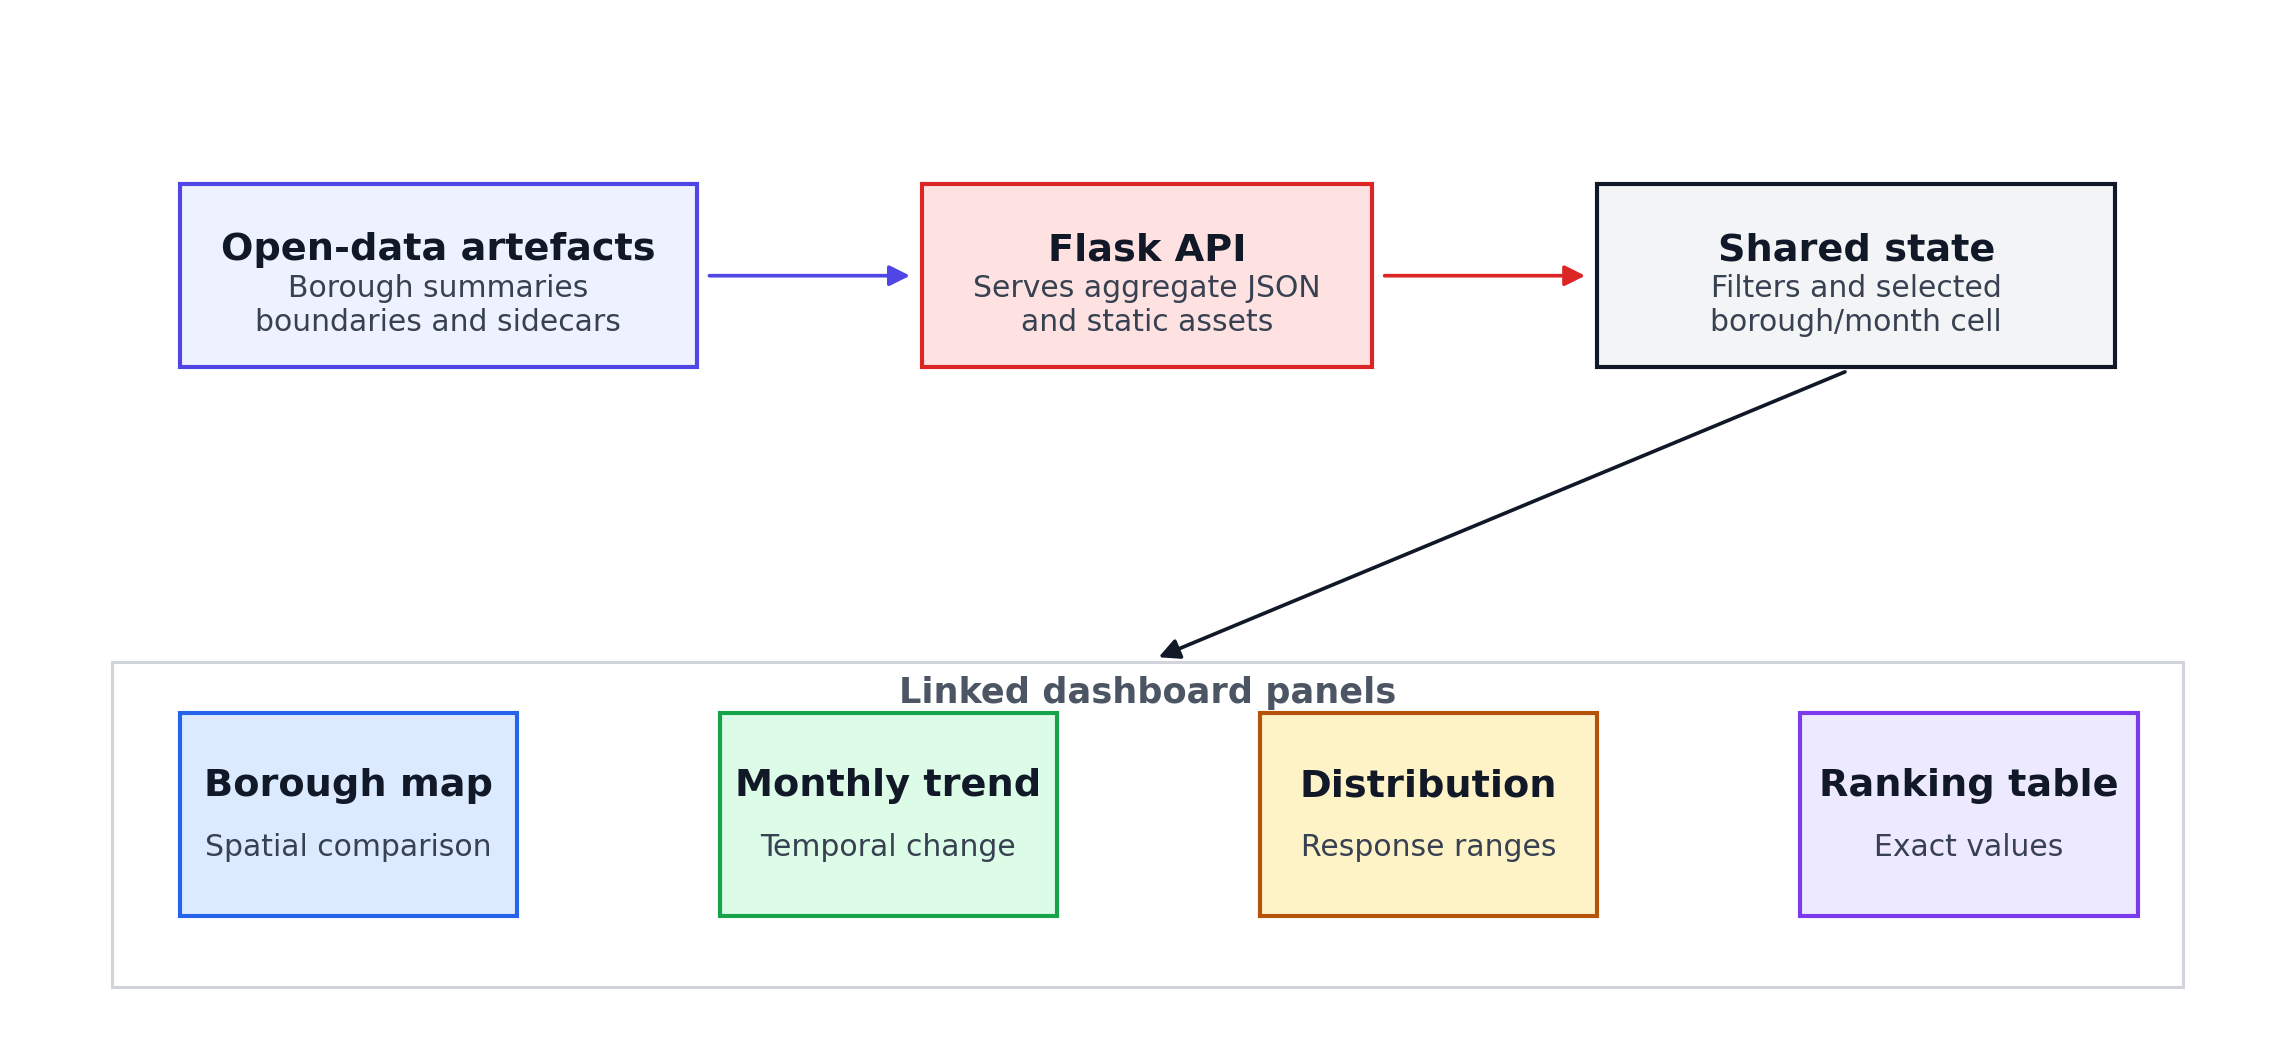
\includegraphics[width=\textwidth]{figures/early_context/fig_linked_view_wireframe.png}
\caption{Linked-view dashboard structure. The schematic shows how the filter state and borough selection propagate through the map, monthly trend, response distribution, and ranking-table panels.}
\label{fig:linked-view-wireframe}
\end{figure}

The backend / front-end split follows from N1--N3 of \S4.2: an open-data, single-laptop, browser-rendered system rules out a separate compute server, but a pure-static deployment would have to ship the canonical 66\,MB Excel (or its $\geq$\,40\,MB parquet derivative) to every browser. The adopted hybrid architecture utilizes a Flask process that loads the borough summary parquet once at startup and serves either pre-aggregated JSON or filter-narrowed slices over the same \path{/api/borough_summary} endpoint; the same Flask process serves the D3 dashboard's static assets and the borough-boundary GeoJSON from the same origin, which removes the need for cross-origin headers and makes the system executable via a single autonomous Flask instance. The first-iteration front-end issues a single unfiltered fetch at startup ($\approx$\,1.0\,MiB JSON, the full 2{,}574-row aggregate) and applies further filters client-side; an explicit borough-only filter would return $\approx$\,31\,KiB. The endpoint supports both patterns so a future front-end iteration can switch to per-state-change fetches without an API change. The per-incident canonical table is never exposed through the HTTP surface --- only aggregations by borough, month, and incident group from \S5.2 leave the backend --- which is both a privacy posture (no precise coordinates over the wire) and a payload-size posture (1\,MiB aggregate JSON, against $\geq$\,40\,MB if the canonical were served whole).

Commercial BI platforms such as Tableau, Power BI, and ArcGIS Online were considered as cheaper implementation paths. A custom build was selected because recorded denominators, Wilson intervals, small-sample and partial-month flags, and API notes needed to be implemented and tested with the data schema. N1--N3 also favour a browser interface that runs locally without a paid desktop or hosted GIS workspace, while N4 favours script-based rebuilds and provenance sidecars. D3 makes the shared selection state and encoding choices available for inspection in the source.

\subsection{Encoding Choices and Their Justification}

Encoding choices follow the \S\ref{sec:background-va} working definitions. The borough choropleth encodes the author-derived share above 360 seconds through a sequential colour scale. The temporal pane aligns incident count and that diagnostic on a common time axis, supporting Yi et al.'s \emph{Connect} category~\cite{yi2007}. The distribution pane shows median-to-p95 ranges with six minutes as a reference line; it does not relabel the reference as an incident-level service target. A full quantile-dotplot remains future work after Hullman et al.~\cite{hullman2015hops}.

The interface separates four issues that were previously grouped under ``uncertainty''. Response variability is shown by median-to-p95 ranges. Response-time missingness is handled by the recorded denominator. Finite-sample uncertainty is shown by 95\% Wilson intervals and a recorded-$n<30$ flag. Coordinate suppression and rounded-point displacement are reported only for point/grid analysis, because they do not condition borough aggregates. February 2026 is marked partial rather than treated as a complete monthly observation.

\subsection{Station Context and Data Requirements}

The project uses two station references: assignment footprints derived from historical incident responsibility patterns (\S5.5), and postcode-geocoded historical public addresses (\S5.6 D1). Both use straight-line distance. The optimisation literature from Church and ReVelle~\cite{church1974} through later surveys and applications \cite{goldberg2004, reconfig2023, beijing2021, ocmola2018} also requires verified locations, road travel times, station capacity, dispatch rules, and live availability. Those inputs are unavailable here. Figure~\ref{fig:station-evidence-boundary} distinguishes the current comparison from the additional data needed for an operational coverage study.

\begin{figure}[H]
\centering
\resizebox{\textwidth}{!}{%
\begin{tikzpicture}[
    ebox/.style={draw, rounded corners=1.5pt, align=center, text width=3.6cm, font=\scriptsize, inner sep=4pt},
    arr/.style={-{Stealth[length=2.0mm]}, line width=0.45pt}
]
\node[ebox, fill=green!8, draw=green!50!black] (fp) at (0,0) {\textbf{Assignment footprint}\\[2pt] historical incident responsibility derived from \texttt{IncidentStationGround}};
\node[ebox, fill=blue!8, draw=blue!55!black] (pa) at (0,-2.9) {\textbf{Public station address}\\[2pt] postcode-geocoded historical address};
\node[ebox, fill=orange!9, draw=orange!65!black, text width=4.0cm] (cmp) at (5.9,-1.45) {\textbf{Current comparison}\\[2pt] straight-line distances between footprint centroids, borough demand centroids, and public-address points};
\node[ebox, fill=red!8, draw=red!60!black] (nc) at (11.8,-1.45) {\textbf{Additional modelling}\\[2pt] road travel times, capacity, dispatch rules, and live availability};
\draw[arr] (fp.east) .. controls +(right:9mm) and +(left:9mm) .. ([yshift=2.5mm]cmp.west);
\draw[arr] (pa.east) .. controls +(right:9mm) and +(left:9mm) .. ([yshift=-2.5mm]cmp.west);
\draw[arr, draw=orange!65!black] (cmp.east) -- (nc.west);
\draw[red!70!black, dashed, line width=0.6pt] (9.15,1.1) -- (9.15,-4.2);
\node[font=\scriptsize\bfseries, text=red!70!black] at (9.15,1.45) {scope limit};
\node[draw, rounded corners=1.5pt, fill=gray!8, align=center, text width=15.0cm, font=\scriptsize, inner sep=4pt, anchor=north] at (5.9,-4.7) (miss) {\textbf{Operational coverage requires:} verified current locations, a road network and travel times, station capacity, dispatch rules, and live availability.};
\end{tikzpicture}}
\caption{Station-data scope. The current analysis compares straight-line distances; operational coverage would additionally require verified locations, travel times, capacity, dispatch rules, and live availability.}
\label{fig:station-evidence-boundary}
\end{figure}

\subsection{Evaluation Plan}

Evaluation occupies the \emph{Evaluating User Experience (UE)} scenario of Lam et al.'s seven-scenario taxonomy~\cite{lam2011}, supplemented by light task-based elements where the research questions admit observable behaviour. The heuristic walk-through draws on the exploration, communication, abstraction, and cognitive-fit concerns of \S\ref{sec:lit-va}--\S\ref{sec:lit-uncertainty}. The task and uncertainty probes test whether a comparison path preserves denominator, coordinate, mobilisation, and station-context caveats. A controlled comparison against a static baseline remains out of scope and is named as future work in \S8.3.
